\documentclass{article}

\usepackage[T1]{fontenc}
\usepackage{lmodern}
\usepackage{graphicx}
\usepackage[margin=1.25in]{geometry}
\graphicspath{ {C:/Users/brent/Downloads/} }
\usepackage[utf8]{inputenc} % allow utf-8 input
\usepackage[T1]{fontenc}    % use 8-bit T1 fonts
\usepackage{hyperref}       % hyperlinks
\usepackage{url}            % simple URL typesetting
\usepackage{booktabs}       % professional-quality tables
\usepackage{amsfonts}       % blackboard math symbols
\usepackage{nicefrac}       % compact symbols for 1/2, etc.
\usepackage{microtype}      % microtypography
\graphicspath{{latex_images}}

\title{Software Tool: Housing Price Visualization}

\author{%
  Brent Christy, Jinyu Liu, Brianna Outen \\
  Northeastern University\\
  Boston, MA 02115 \\
  \texttt{christy.b@northeastern.edu, liu.jinyu@northeastern.edu, outen.b@northeastern.edu} \\
}

\begin{document}

\maketitle

\begin{abstract}
  
Jinyu

\end{abstract}

\section{Problem and Background}
Brianna

\section{Tool Description and Features}
Brianna


\section{Software Architecture}
Jinyu

\section{Insights and Observations}
There are a wide variety of use cases for visualizing aggregated housing data on a map. The spacial mapping of housing information can allow for many comparisons to be made, whether it be across time for observing how quickly prices are changing, or across area for comparing how different prices are in different areas. In the following subsections, several situations will be described where the visualization tool can be used to make decisions and analyze data.

\subsection{Deciding on an Area to Live}
An interesting use case for the software tool is using it to identify an area of the country to live in. A good example is a couple moving to the Boston area. The couple doesn't know much about the area but does know that they have a budget of around \$800,000 to spend on their house. The couple can use our software tool to zoom in on the Boston area to begin. They then can set a static colorbar limit from \$500,000 to \$700,000 on the tool and look around the area. A range of \$500,000 to \$700,000 will show the areas of the region whose median home price is in the range. A bright yellow color will tell the couple that the majority of homes in that zip code are going to be out of their price range. A darker blue color will tell the couple that the homes in that area are probably below their price range. 

\begin{center}
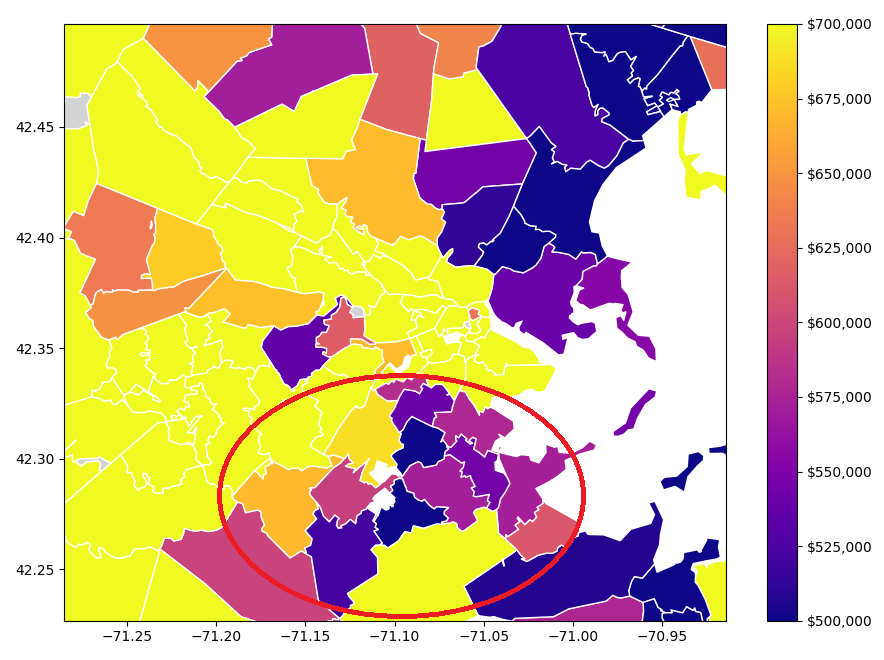
\includegraphics[scale=0.5]{five_hundred_to_seven_hundred.png} 
\end{center}

As can be seen in the color bar in the example above, the range is from \$500,000 to \$700,000. The area that is circled in red south of the city of Boston is a likely area that the couple would identify as a possible place to live. There are many shades between the minimum and maximum in this area and it appears to be a reasonable commute to the city from here. Having identified a reasonable region to live in, the couple may be able to go to a real estate agent with their ideal region picked out, making the process much quicker.

\subsection{Identifying Gentrification}
Another case that the tool could be used for is identifying areas that are becoming gentrified. The feature of the tool that will be used here is adjusting the time being shown. Since the tool has data going all the way back to the year 1996, it is easy to compare how different housing prices are across time periods. This is especially useful for identifying regions of metro areas that are being gentrified. The dynamic color bar is useful for this application.


\begin{center}
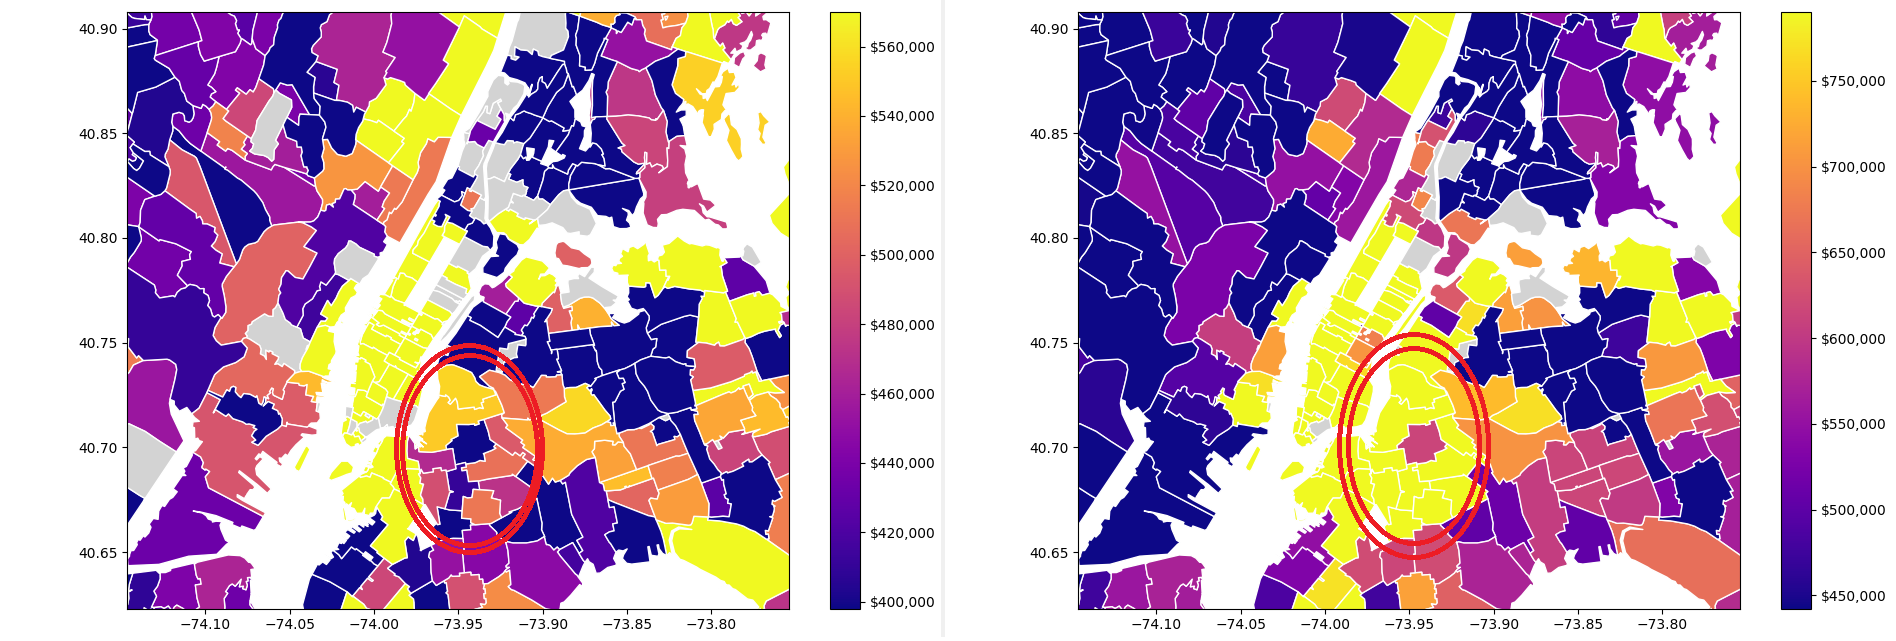
\includegraphics[scale=0.3]{2006_2021_nyc.png} 
\end{center}


The area in red circled above defines an area of Brooklyn including Greenpoint, Williamsburg, and Bushwick. These are areas of Brooklyn well known in the last ten years to have an influx of younger people moving to the area. With younger people moving to the area, the cost of rent and homes will go up accordingly. This can be seen in the images above. Since the color bar is relative in this case, it shows the cost of the homes relative to the areas around it. In the image on the left, 2006, the areas in the circle are darker shades, showing that they are relatively lower than the areas surrounding it. In 2021, the image on the right, you can see that all of the zip codes in the area other than one are now in the highest range of the map, in bright yellow. This tells us that the prices of these homes have moved relatively from being average priced homes in the area to being in the upper percentage of cost in the area. This approach could be taken analyzing areas of any metro area in order to identify and address issues of gentrification.


\section{Future Work}
There are many ways that this work could be expanded in the future. Because of the flexible architecture of the tool, it would be easy to add any kind of numerical metric to the map. Rather than mapping housing prices, something like number of crimes could be visualized as well. The scale would be minimum and maximum crimes committed rather than minimum and maximum of the median home prices. In addition to these, metrics could also be combined to show more advanced statistics such as housing price versus commute time.

There are other features that could have been added to the map to make it more user friendly. Regional markers could be added to help users identify areas of the country better. Regional markers that could be added include cities, towns, and other popular landmarks. In order to make the tool more useful for house hunters, information that could be interesting to a home buyer could be added when clicking on the zip code, such as the schools in the area or community resources.


\end{document}